\textbf{Multiple Choice}. Clearly mark the correct answer for each of the following by completely filling in the appropriate bubble or box. No justification is needed.
\begin{questions}

\question[3]  Which of the following functions have inverse functions? [Select \textbf{MULTIPLE}]
    \begin{multicols}{2}
    \checkboxchar{\Large$\Box$}\begin{checkboxes}
    
    \choice \hspace{-3em} A. \phantom{a}\vspace{-.7cm}
    
        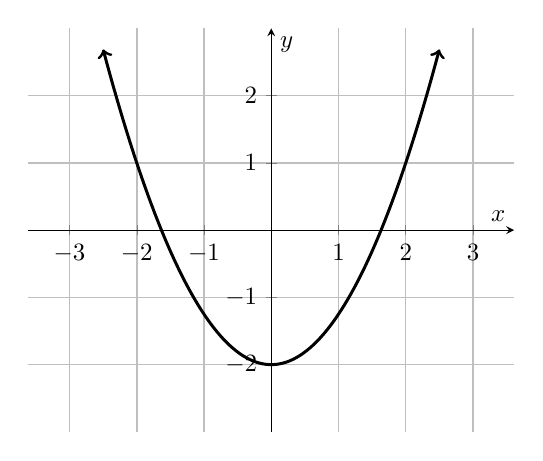
\begin{tikzpicture}[scale = .9]
          \begin{axis}[
            domain=-2.5:2.5,
            samples=100,
            xmin=-3, xmax=3,
            ymin=-3, ymax=3,
            axis equal,
            axis lines=middle,
            xlabel={$x$},
            ylabel={$y$},
            xtick={-3,-2,-1,0,1,2,3},
            ytick={-2,-1,0,1,2},
            grid=both,
            minor grid style={dotted},
            major grid style={semithick}
          ]
             \addplot[black, very thick, <->] {.75*x*x-2};
            \end{axis}
        \end{tikzpicture}
        
        \vspace{-1cm}
        \choice \hspace{-3em} B.\phantom{a}
        
          \begin{tikzpicture}
                \foreach[count=\i] \lseti/\lsetmi in {A/{x,y,z,w},B/{a,b,c}} {
                \begin{scope}[local bounding box=\lseti, x=3cm, y=.5cm]
                \foreach[count=\j] \lj in \lsetmi {
                    \node[minimum width=1em] (n-\j-\lseti) at (\i,-\j) {\lj};
                }
                \end{scope}
                \node[ellipse, draw, fit=(\lseti), 
                label={[name=l-\lseti]above:$\lseti$}] {};
                }
                \draw[->] (n-1-A) -- (n-2-B);
                \draw[->] (n-2-A) -- (n-1-B);
               % \draw[->] (n-3-A) -- (n-1-B);
                \draw[->] (n-3-A) -- (n-3-B);
                \draw[->] (n-4-A) -- (n-3-B);
            \end{tikzpicture}
    \columnbreak
    
        \choice \hspace{-3em} C. \phantom{a}\vspace{-.7cm}
        
        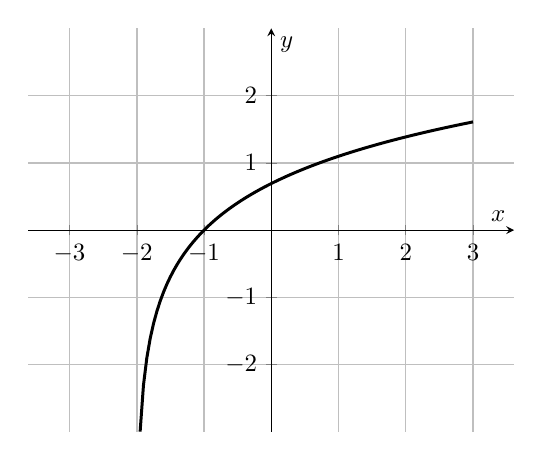
\begin{tikzpicture}[scale = .9]
          \begin{axis}[
            domain=-1.95:3,
            samples=100,
            xmin=-3, xmax=3,
            ymin=-3, ymax=3,
            axis equal,
            axis lines=middle,
            xlabel={$x$},
            ylabel={$y$},
            xtick={-3,-2,-1,0,1,2,3},
            ytick={-2,-1,0,1,2},
            grid=both,
            minor grid style={dotted},
            major grid style={semithick}
          ]
             \addplot[black, very thick] {ln(x+2)};
            \end{axis}
        \end{tikzpicture}
        \vspace{1cm}
    
        \choice \hspace{-3em} D. \phantom{a}\vspace{-.7cm}
    
        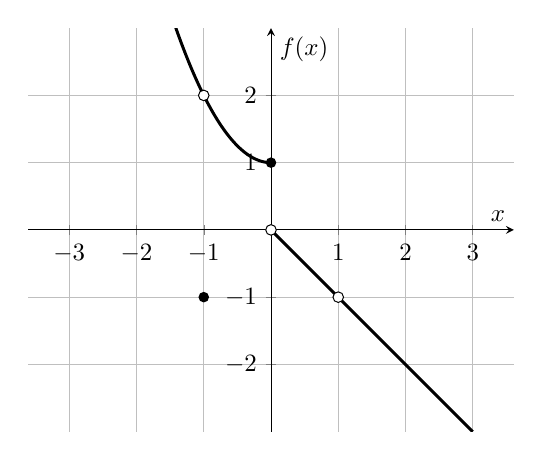
\begin{tikzpicture}[scale = .9]
        \begin{axis}[
            axis lines = middle,
            xlabel = {$x$},
            ylabel = {$f(x)$},
            grid = both,
            xmin = -3, xmax = 3,
            ymin = -3, ymax = 3,
            xtick={-3,-2,-1,0,1,2,3},
            ytick={-2,-1,0,1,2},
            samples = 100,
            axis equal,
        ]
        
        % Plot f(x) = x^2 + 1 for x < 0, excluding x = -1 for the hole
        \addplot[domain=-3:-1.01, black, very thick] {x^2 + 1};
        \addplot[domain=-0.99:0, black, very thick] {x^2 + 1};
    
        % Plot f(x) = -x for x > 0, excluding x = 1 for the hole
        \addplot[domain=0.01:3, black, very thick] {-x};
    
        % Draw the holes
        \node at (axis cs:-1,2) [circle,draw,black,fill=white,inner sep=1.5pt] {};
        \node at (axis cs:1,-1) [circle,draw,black,fill=white,inner sep=1.5pt] {};
        \node at (axis cs:0,0) [circle,draw,black,fill=white,inner sep=1.5pt] {};
    
        % Plot the special point at (-1, -1)
        \node at (axis cs:-1,-1) [circle,fill=black,inner sep=1.5pt] {};
        \node at (axis cs:0,1) [circle,fill=black,inner sep=1.5pt] {};
        \end{axis}
    \end{tikzpicture}
        
        \end{checkboxes}
    \end{multicols}
\vfill
%\todo{Make the checkboxes all in the upper left corner}

\question[3]
    A polynomial has a leading term of $-3x^4$. What is the end behavior of this polynomial? [Select \textbf{ONE}]
    \begin{choices}
        \choice \chooseone As $x\to +\infty$, $y\to -\infty$ and as $x\to -\infty$, $y\to +\infty$
        \choice \chooseone As $x\to +\infty$, $y\to +\infty$ and as $x\to -\infty$, $y\to +\infty$
        \choice \chooseone As $x\to +\infty$, $y\to -\infty$ and as $x\to -\infty$, $y\to -\infty$
        \choice \chooseone As $x\to +\infty$, $y\to +\infty$ and as $x\to -\infty$, $y\to -\infty$
        \choice \chooseone None of the above
    \end{choices}
\vfill

\newpage
\question[3]
    Consider a parabola $f(x)=ax^2+bx+c$. If the graph of $y=ax^2+bx+c$ intersects the $x$-axis at two separate points, what can we say about the roots of $f(x)$? [Select \textbf{ONE}]
    \begin{choices}
        \choice \chooseone There are two real roots of $f(x)$
        \choice \chooseone There may be either one or two real roots of $f(x)$, and we need more information to know.
        \choice \chooseone There are two complex roots of $f(x)$
        \choice \chooseone There is exactly one real root of $f(x)$
        \choice \chooseone None of the above.
    \end{choices}
\vspace{3em}


\question[3] %diego, I'm going to make some grammatical changes to this question
    Colt works as a stuntman in action movies. Let $x$ be the number of hours he works. The equation for his money earned (in dollars) is given by
    \[ P(x) = 10 x-8.\]
    What is the rate of change and what does it represent? [Select \textbf{ONE}]
    \begin{choices}
        \choice \chooseone He earns 10 dollars per hour of work.
        \choice \chooseone He does 10 stunts per hour.
        \choice \chooseone He loses 8 dollars per hour of work.
        \choice \chooseone $x=\dfrac{5}{4}$
        \choice \chooseone None of the above.
    \end{choices}



\newpage
% \hspace{-.5in}Free answer section. Work must be shown to get credit for any answer. Partial credit may be given even for incorrect final answers, so show your work.

%     \question %composition domain
%     Let $f(x)=\sqrt{x}+x$ and $g(x)=\frac{1}{x}+1$. 
%     \begin{parts}
%         \part[5] Find $f(x)\cdot g(x)$ and its domain.
%         \vspace{7cm}
%         \part[4] Find $f\circ g(x)=f(g(x))$. You do not need to simplify.
%         \vspace{5cm}
%         \part[4] Find $g\circ g(x)=g(g(x))$. You do not need to simplify.
%         \vspace{5cm}
%  \end{parts}

% \newpage

\begin{comment}
\question[12] Here is a graph of the parent function $f(x)= \sqrt{x}$.
\todo{By Decree of Travis: We will punt this question and come back to it.}
        \begin{center}
            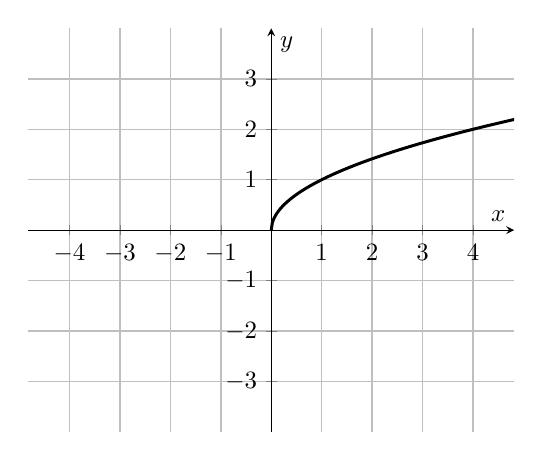
\begin{tikzpicture}[scale=0.9]
                          \begin{axis}[
                            domain=0:5,
                            samples=100,
                            xmin=-4, xmax=4,
                            ymin=-4, ymax=4,
                            axis equal,
                            axis lines=middle,
                            xlabel={$x$},
                            ylabel={$y$},
                            xtick={-4,-3,-2,-1,0,1,2,3,4},
                            ytick={-3,-2,-1,0,1,2,3},
                            grid=both,
                            minor grid style={dotted},
                            major grid style={semithick}
                          ]
                             \addplot[black, very thick, samples=250] {sqrt((x))};
                            \end{axis}
            \end{tikzpicture}
        \end{center}

Match each function child function below to its graph. Write the letter of the corresponding graphs in the boxes next to the functions below.

    \begin{multicols}{2}
        \begin{enumerate}
            \item[(A)] 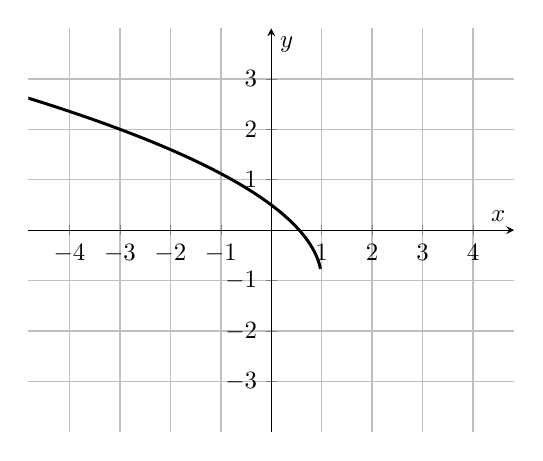
\begin{tikzpicture}[scale=0.9]
                      \begin{axis}[
                        domain=-5:1,
                        samples=100,
                        xmin=-4, xmax=4,
                        ymin=-4, ymax=4,
                        axis equal,
                        axis lines=middle,
                        xlabel={$x$},
                        ylabel={$y$},
                        xtick={-4,-3,-2,-1,0,1,2,3,4},
                        ytick={-3,-2,-1,0,1,2,3},
                        grid=both,
                        minor grid style={dotted},
                        major grid style={semithick}
                      ]
                         \addplot[black, very thick, samples=250] {1.5*sqrt(-x+1)-1};
                         %\node at (axis cs: 2,1.5) [anchor=north west] {$\mathbf{f(x)}$};
                        \end{axis}
                \end{tikzpicture}
                
            \item[(B)] 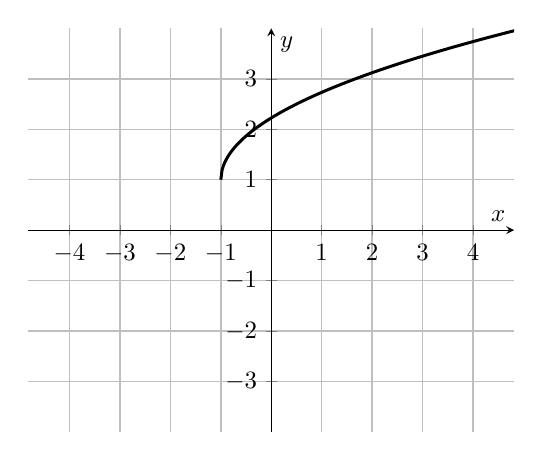
\begin{tikzpicture}[scale=0.9]
                      \begin{axis}[
                        domain=-1:5,
                        samples=100,
                        xmin=-4, xmax=4,
                        ymin=-4, ymax=4,
                        axis equal,
                        axis lines=middle,
                        xlabel={$x$},
                        ylabel={$y$},
                        xtick={-4,-3,-2,-1,0,1,2,3,4},
                        ytick={-3,-2,-1,0,1,2,3},
                        grid=both,
                        minor grid style={dotted},
                        major grid style={semithick}
                      ]
                         \addplot[black, very thick, samples=250] {sqrt((3/2)*(x+1))+1};
                         %\node at (axis cs: 2,1.5) [anchor=north west] {$\mathbf{f(x)}$};                 
                        \end{axis}
                \end{tikzpicture}
                
                
            \item[(C)] 
            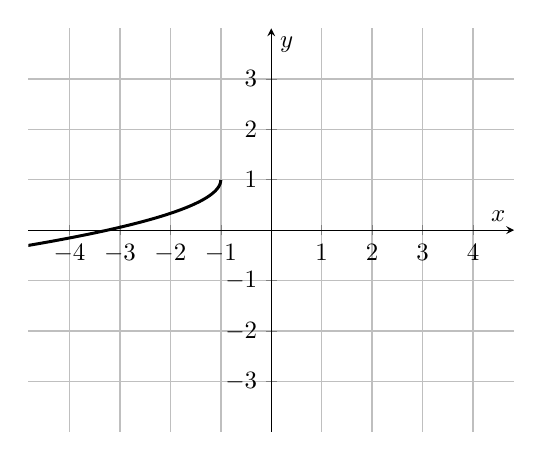
\begin{tikzpicture}[scale=0.9]
                      \begin{axis}[
                        domain=-5:-1,
                        samples=500,
                        xmin=-4, xmax=4,
                        ymin=-4, ymax=4,
                        axis equal,
                        axis lines=middle,
                        xlabel={$x$},
                        ylabel={$y$},
                        xtick={-4,-3,-2,-1,0,1,2,3,4},
                        ytick={-3,-2,-1,0,1,2,3},
                        grid=both,
                        minor grid style={dotted},
                        major grid style={semithick}
                      ]
                         \addplot[black, very thick, samples=500] {-(2/3)*sqrt(-x-1)+1};
                         %\node at (axis cs: 2,1.5) [anchor=north west] {$\mathbf{f(x)}$};                 
                        \end{axis}
                \end{tikzpicture}
                
            \item[(D)] 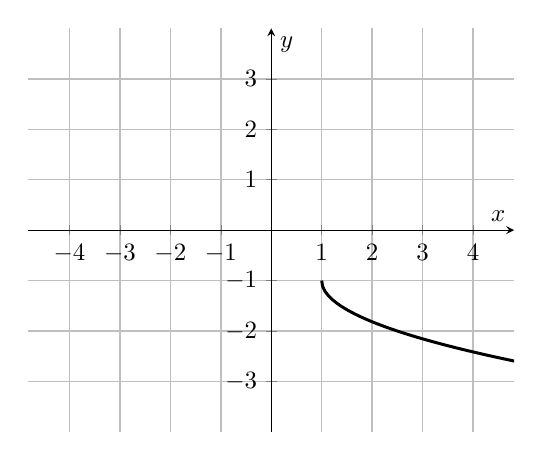
\begin{tikzpicture}[scale=0.9]
                      \begin{axis}[
                        domain=1:5,
                        samples=100,
                        xmin=-4, xmax=4,
                        ymin=-4, ymax=4,
                        axis equal,
                        axis lines=middle,
                        xlabel={$x$},
                        ylabel={$y$},
                        xtick={-4,-3,-2,-1,0,1,2,3,4},
                        ytick={-3,-2,-1,0,1,2,3},
                        grid=both,
                        minor grid style={dotted},
                        major grid style={semithick}
                      ]
                         \addplot[black, very thick, samples=250] {-1*sqrt((2/3)*(x-1))-1};
                         %\node at (axis cs: 2,1.5) [anchor=north west] {$\mathbf{f(x)}$};
                        \end{axis}
                \end{tikzpicture}
        \end{enumerate}
    \end{multicols}

   

    \begin{multicols}{2}
        \Scale[5]{\boxed{ \hspace{.1cm}}} $\displaystyle -\frac{2}{3}\sqrt{-x-1}+1$\vspace{0.5cm}
        
        \Scale[5]{\boxed{ \hspace{.1cm}}} $\displaystyle -\sqrt{\frac{2}{3}(x-1)}-1$ \vspace{0.5cm}
           
        \Scale[5]{\boxed{ \hspace{.1cm}}} $\displaystyle \sqrt{\frac{3}{2}(x+1)}+1$ \vspace{0.5cm}
        
        \Scale[5]{\boxed{ \hspace{.1cm}}} $\displaystyle \frac{3}{2}\sqrt{-x+1}-1$ \vspace{0.5cm}
    \end{multicols}



\end{comment}






\newpage
\hspace{-.5in}\textbf{Short Answer}. Show your work; partial credit may be awarded.

\question Consider the two graphs below of $f(x)$ and $g(x)$.
\begin{multicols}{2}
    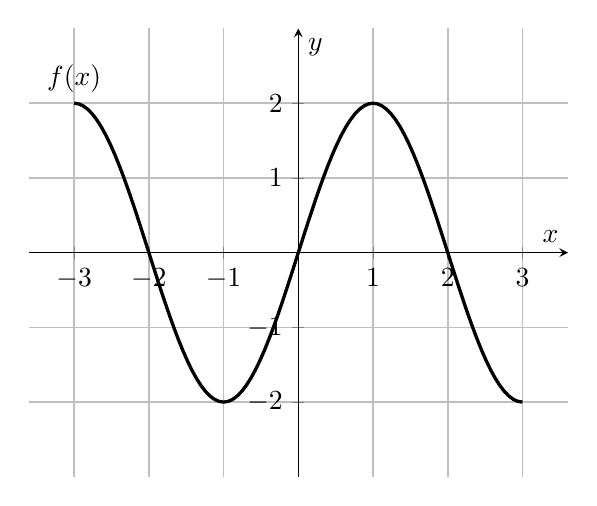
\begin{tikzpicture}
      \begin{axis}[
        domain=-3:3,
        samples=100,
        xmin=-3, xmax=3,
        ymin=-3, ymax=3,
        axis equal,
        axis lines=middle,
        xlabel={$x$},
        ylabel={$y$},
        xtick={-3,-2,-1,0,1,2,3},
        ytick={-2,-1,0,1,2},
        grid=both,
        minor grid style={dotted},
        major grid style={semithick}
      ]
         \addplot[black, very thick] {2*sin(deg(0.5*pi*x))} node[pos=0, above] {$f(x)$};
        \end{axis}
    \end{tikzpicture}

    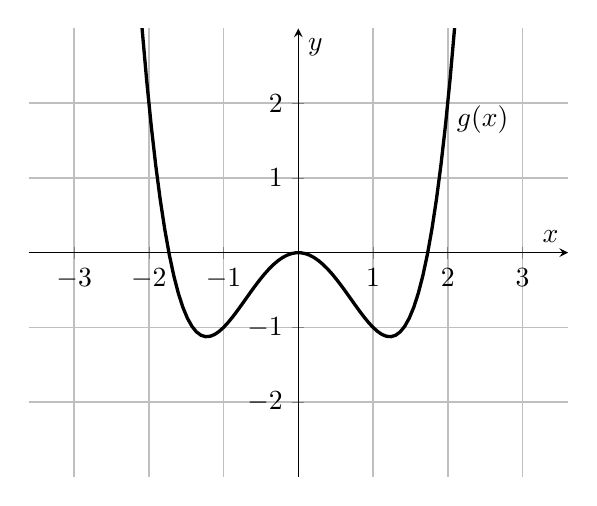
\begin{tikzpicture}
      \begin{axis}[
        domain=-3:3,
        samples=100,
        xmin=-3, xmax=3,
        ymin=-3, ymax=3,
        axis equal,
        axis lines=middle,
        xlabel={$x$},
        ylabel={$y$},
        xtick={-3,-2,-1,0,1,2,3},
        ytick={-2,-1,0,1,2},
        grid=both,
        minor grid style={dotted},
        major grid style={semithick}
      ]
         \addplot[black, very thick] {0.5*x*x*x*x -1.5*x*x } node[pos=.58, right] {$g(x)$};
        \end{axis}
    \end{tikzpicture}
\end{multicols}

    \begin{parts}
    \part[3] Find $(g-f)(1) = \Scale[5]{\boxed{ \hspace{.3cm}}}$
    \vspace{.5cm}
    \part[3] Find $g\circ f (3) = \Scale[5]{\boxed{ \hspace{.3cm}}}$
    \vspace{.5cm}
\end{parts}
\vfill

\question[10] Sketch the graph of the function
    \vspace{-0.2cm}
    \begin{equation*}
        f(x)=(x+1)^3(x-1)^2(x-3).
    \end{equation*}
 
\begin{tikzpicture}
\begin{axis}[
  width= \textwidth,
  height= .6\textwidth,
  axis lines=middle,
  %grid=major,
  xmin=-4.5,
  xmax=4.5,
  ymin=-4,
  ymax=4,
  xlabel=$x$,
  ylabel=$y$,
  xtick={-4,-3,...,4},
  ytick=false,%{-4,-3,...,4},
  tick style={very thick},
  legend style={
  at={(rel axis cs:0,1)},
  anchor=north west,draw=none,inner sep=0pt,fill=gray!10}
]
\end{axis}
\end{tikzpicture}


% \vfill

\newpage
\question %Building Polynomials

    \begin{parts}
    \part[6] Find the polynomial $h(x)$ of  least possible degree with \underline{integer coefficients} %and a repeated root $1 + 2i$ with multiplicity $2$ such that $f(1) = 50$ and $f(3) = 0$. %We have said the complex roots aren't on this exam
    that has a repeated root of 3 with multiplicity 2 and a root of $\sqrt{2}$ such that $h(0)=-36$.
    
    (You may leave your answer as a product of linear factors.)
    
    %Grading Notes: the extra root at -sqrt(2) worth at most 1 point
    
    \vfill\vfill\vfill
    
    %\vfill
    \part[4] What is the leading term of the polynomial and what is the degree of the polynomial?
    %Determine all the roots of $f(x)$ and their corresponding multiplicity.
    %\todo{Could we change this part to asking: what is the degree of $f$, what is the leading term, and what is the constant term?}
    \vfill
    %\part[2]
    \end{parts}
    

    
% \end{parts}



\newpage

\question[10]  
    Perform the polynomial division below, and identify the quotient and remainder.
    %\todo{This needs more space: put on its own page?}
    
    % \begin{parts}
    
    % \part[5] 
    % $\left(4 x^5-6 x^3-8 x+5\right) \div(2 x-4)$
    
    % \vfill
    
    % \part[5] 
    \begin{equation*} %Changed the x^2 term to 10x^2 instead of 2x^2 to avoid flustering students with 4*18
        \left(5 x^4-3 x^3+10 x^2-1\right) \div\left(x^2+4\right)
    \end{equation*}
    



\newpage

\question
    Consider two functions $f(x) = \sqrt{x+5}$ and $g(x) = x^2 -9$.
    
    \begin{parts}
    \part[2] Compute $f\cdot g(x)$.
    
    \vfill
        
    \part[4] Let $h(x) = \dfrac{f(x)}{g(x)}$. Compute $h(4)$ and the domain of $h(x).$ 
     
    \vfill\vfill
    
    
    \part[4] Compute $f\circ g(x)$ and find its domain.
    
    \vfill\vfill\vfill
    \end{parts}

\newpage
\question 
    For each of the following functions, find the inverse function and its domain, or state that the inverse does not exist.

    \begin{parts}
    % \part[3] $f(x) = (x-2)^3 + 1$
    
    % \vfill
    \part[5] $g(x) = \dfrac{13}{1+x}$
    \vfill
    \part[5] $h(x) = x^2 - 4x$
    \vfill
    %\part[3] Draw the graph of the inverse of the red function. The graph of $y=x$ is provided for reference.
    
    %
    \end{parts}

\newpage
\question 
    A pharmaceutical company has a process for creating a drug from bacteria. If  $x$ is the number of bacteria (in millions), the amount of drug (in grams) created is given by the model 
    \[D(x)=20x-4x^2.\]
    \begin{parts}
        \part[2] How many grams of the drug is created from 2 (million) bacteria?
        \vfill
        \part[3] What number(s) of bacteria would result in \underline{none} of the drug being created? % "how many" "0 grams of the drug"
        \vfill
        \part[5] What is the maximum amount of the drug that can be created, and how many bacteria (in millions) are required to create it? %"number of grams"
        \vfill\vfill
    \end{parts}
    %\todo{Should this be phrased as a word problem or a modeling question? I see benefits to isolating the skill and to applying it.}

\newpage

% \question There is a petri dish which contains planarians. At 10am there were two planarians. The planarians triple in population every two hours. 

% \begin{enumerate}
%     \item Find a function $P(t)$ that models the population of the planarians after $t$ hours.

%     \item What is the population of the planarians at 2:30pm on the same day? (You do not have to simplify your answer.)
% \end{enumerate}

% \newpage
% %4.2 Question. I'm assuming this will be bumped to the next exam (if not this should be heavily modified)
% %Also, logarithms aren't covered until after section 4.2
% \question In a different petri dish a group of scientists are trying to develop a treatment to stop the planarians from growing. They find, after starting with a petri dish containing 1000 planarians, that 3 hours after applying the treatment there are 200 planarians. 

% \begin{enumerate}
%     \item Find a function $P(t)$ that models the population of the planarians after $t$ hours. (Leave the value for $r$ in terms of a $\log$) \todo{We don't cover logarithms until after section 4.2. \textbf{See comment on line 297}}

%     \item Upon more studies the scientists find that the number of planarians in a petri dish $t$ hours after treatment is best modeled by the function $P(t) = 800 e^{0.5\ln(1/3)t}$. Is this function increasing or decreasing? Explain why?

%     \item Using this new model when will there be $100$ planerians in the petri dish? (Leave your answer in terms of a $\log$)
% \end{enumerate}


% \begin{comment}
% Alternate 4.2 question
%     \question In a different petri dish a group of scientists is developing a new sub-species of super-planarians that can produce even faster than planarians. They determine that the growth of the super-planarians can be modeled by the exponential equation $P(t) = Ce^{rt}$ where $t$ is time in hours. At the start of the experiment there are 150 super-planarians in the petri dish and by the third hour of the experiment there are 1200 super-planarians in the petri dish.


% \begin{enumerate}
%     \item Find a function $P(t)$ that models the population of the planarians after $t$ hours. (You may leave the value for $r$ in terms of a $\log$)

%     \item When will there be 10,000 super-planarians in the petri dish.(Leave it in terms of a log. If you did not get an answer for part 1 use the equation $P(t) = 30e^{\ln{5}t}$) 
% \end{enumerate}
% \end{comment}


%Yuchen 3.4Inequalities

\newpage
\question %\textbf{[Section 3.4\&3.5]} 
    Let %$f(x)=2x^3-10x^2+13x-5$. %Roots x= 1, 2\pm sqrt{3/2}
    %
    %or 
    $f(x)=10x^3-19x^2+11x-2.$ %Roots x=1, 2/5 and 1/2
    
    %or $f(x) = 6x^{3}-19x^{2}+19x-6$. %\todo{This has no rational roots}
    %Owen here: should it be 16 rather than 19?
    %{\color{red}Yuchen: Fixed. Rational roots: 1, 2/3, 3/2.}
    \begin{parts}
    \part[2] List all possible rational roots of $f(x)$ according to the rational root theorem.
    \vfill
    
    \part[8] We know that $f(x)$ has a root at $x=1$. Use this fact to find all the roots of $f(x)$.
    
    \vfill\vfill\vfill
    
    \part[2] Write $f(x)$ as a product of linear factors.
    \vfill
    \end{parts}

\newpage


%%%%%%%%%%%%%%%%% 2.6 Transformations John %%%%%%%%%%%%%%%%%%%%%%
\question 

    The following is a graph of the function $f(x)$.
    \vspace{-0.5cm}
        \begin{center}
            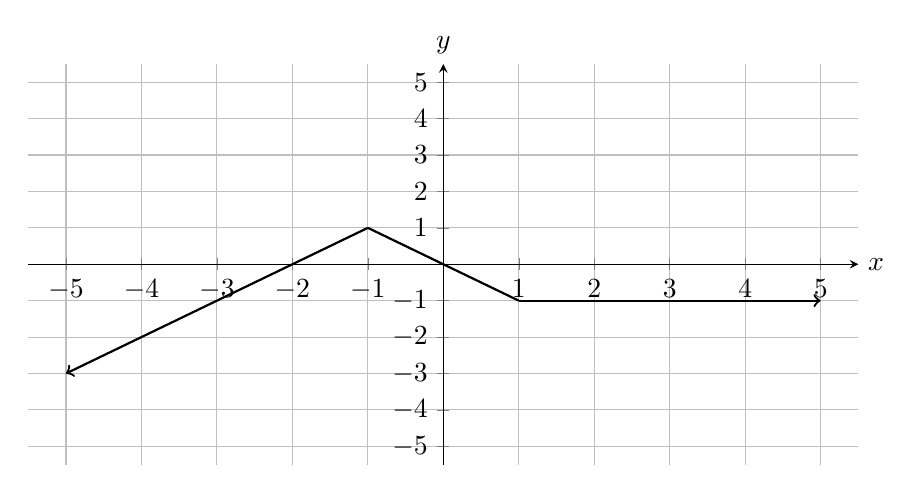
\begin{tikzpicture}
                \begin{axis}[ 
                    width=\textwidth,
                    height=0.55\textwidth,
                    axis lines = center,
                    grid = both,                  % Add a grid          % Number of minor ticks between major ticks
                    xmin=-5.5, xmax=5.5,
                    ymin=-5.5, ymax=5.5,
                    xlabel=$x$, ylabel=$y$,
                    xtick={-5,-4,...,5},          % Set x-axis ticks every 1 unit
                    ytick={-5,-4,...,5},          % Set y-axis ticks every 1 unit
                    samples=300,
                    domain=-5:5,
                    restrict y to domain=-5:5,
                    every axis y label/.style={at={(ticklabel* cs:1)},anchor=south},
                    every axis x label/.style={at={(ticklabel* cs:1)},anchor=west},
                ]
                \addplot[domain=-5:-1, black, thick, <-]{x+2};
                \addplot[domain=-1:1, black, thick, -]{-x};
                \addplot[domain=1:5, black, thick, ->]{-1};
                \end{axis}
            \end{tikzpicture}
        \end{center}
    
        The function $g(x)$ is obtained from $f(x)$ by: shifting $f(x)$ two units to the left, stretching the function vertically by a factor of 3, and shifting 1 unit downward. 
    
        \begin{parts}
            \part[3] Write an algebraic expression describing how $g(x)$ was obtained from $f(x)$:
            \vspace{-0.5em}
            \begin{align*}
                \Scale[1.7]{\boxed{g(x) = \hspace{4cm} }}
            \end{align*} %thank you thank you thank you
            
    
            \part[7] Sketch $g(x)$ on the graph below.
            
        \end{parts}
            \vspace{-0.5cm}
            \begin{center}
                    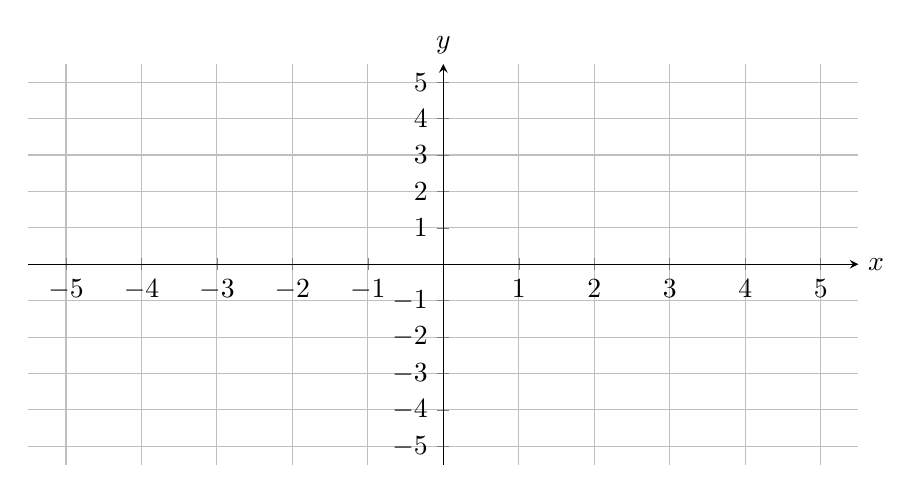
\begin{tikzpicture}
                        \begin{axis}[ 
                            width=\textwidth,
                            height=0.55\textwidth,
                            axis lines = center,
                            grid = both,                  % Add a grid          % Number of minor ticks between major ticks
                            xmin=-5.5, xmax=5.5,
                            ymin=-5.5, ymax=5.5,
                            xlabel=$x$, ylabel=$y$,
                            xtick={-5,-4,...,5},          % Set x-axis ticks every 1 unit
                            ytick={-5,-4,...,5},          % Set y-axis ticks every 1 unit
                            samples=300,
                            domain=-5:5,
                            restrict y to domain=-5:5,
                            every axis y label/.style={at={(ticklabel* cs:1)},anchor=south},
                            every axis x label/.style={at={(ticklabel* cs:1)},anchor=west},
                        ]
                        
                        \end{axis}
                    \end{tikzpicture}
                \end{center}
\end{questions}